\documentclass[12pt,a4paper,titlepage]{article}




\usepackage[utf8]{inputenc}
\usepackage{amsmath}
\listfiles
\usepackage[T1]{fontenc,url}

\usepackage[url=false,isbn=false,style=authoryear,backend=biber,sorting=nyt,maxcitenames=2,uniquelist=false,maxbibnames=12,uniquename=false,texencoding=utf8,bibencoding=utf8]{biblatex}

\renewcommand*{\finalnamedelim}{\addspace\&\space}


\usepackage{etoolbox}
\usepackage{keyval}
\usepackage{import}
%\usepackage{fancyhdr}
%\pagestyle{fancy}
%if biber broken, run <rm -rf `biber --cache`> in terminal

\usepackage{csquotes}
\usepackage[english]{babel}
%\usepackage{babel}
\usepackage{verbatim}
\makeatletter
\patchcmd{\Ginclude@eps}{"#1"}{#1}{}{}
\makeatother
\usepackage[margin=1in]{geometry}
\usepackage{array,booktabs}
\usepackage{ifdraft}
\geometry{a4paper}
\usepackage{graphicx}
\usepackage{import}
\usepackage{latexsym}
\usepackage{grffile}
\usepackage[nolists]{endfloat}
\usepackage{multirow}
\usepackage{tabularx}
%\usepackage{figcaps}
%\usepackage{dontdistribute}
%\usepackage{draftdatetime}
\usepackage[hang,flushmargin]{footmisc}
\renewcommand{\thesection}{\arabic{section}}


\addbibresource{ScottRef.bib}

\usepackage{setspace}

\let\oldtabular\tabular
\renewcommand{\tabular}{\footnotesize\oldtabular}
\DeclareUnicodeCharacter{00A0}{ }
\DeclareUnicodeCharacter{202D}{}
\DeclareUnicodeCharacter{202C}{}


\title{Analyzing policy networks using valued exponential random graph models (ERGMs): Do government-sponsored collaborative groups enhance organizational networks?}
\author{Tyler Scott\\ Evans School of Public Affairs, University of Washington}
\date{June 2014}



\begin{document}

\singlespacing
\maketitle

\begin{abstract}
\doublespacing

This paper examines collaborative management groups from the perspective of policymakers seeking to increase coordination within a policy network. While governments often support collaborative groups as a tool to address perceived network failures such as a lack of coordination, the net impact groups have is unclear. I use valued exponential random graph models (ERGMs) to model relationships of varying strength amongst a regional network of organizations involved in 57 collaborative groups. This provides a unique opportunity to study the interplay between numerous groups and organizations within a large-scale network. Valued ERGMs are a recently developed extension of standard ERGMs that model valued instead of binary ties; thus, this paper also makes a methodological contribution to the policy literature. Findings suggest that participation in collaborative groups does motivate stronger levels of coordination and cooperation amongst organizations network ties between individual organizations; however, this effect is strongest for: (a) organizations that are not already members of another group; and (b) organizations that do not have a pre-existing tie. These results support a transaction-cost based perspective of how government-sponsored collaborative groups can influence network coordination; further, they also provide an empirical example of the Ecology of Games, in which multiple collaborative institutions have interactive effects on one another within a policy network.\\



\noindent
\bf{Keywords}: Collaborative management, policy networks, ERGM, valued networks, network analysis
\end{abstract}

\doublespacing
%\keywords{collaborative management, policy networks, ERGM, network analysis}
\section{\bf\MakeUppercase{Introduction}}

This paper examines how government-sponsored collaborative environmental management groups influence the structure of inter-organizational networks. Collaborative groups continue to grow in popularity as a tool for increasing coordination amongst network actors \parencite{margerum2011}. In theory, government-sponsored groups lower the transaction costs organizations face with regards to forming and maintaining inter-organizational ties by subsidizing a degree of these costs. Thus, participants in groups which facilitate ``principled engagement'' and increase the ``capacity for joint action'' \parencite{emerson2012} are much more likely to engage directly in consultation, planning, or policy implementation with one another as well \parencite{scott2015-a}.

In practice, when viewed at a larger scale it is unclear whether collaborative groups foster a net increase in cooperation and coordination amongst organizations (i.e., more and stronger inter-organizational ties) or whether they simply engender a different pattern of ties with no net change in overall collaborative behavior \parencite{lubell2010,lubell2011}. Recent literature building upon the ``Ecology of Games'' framework \parencite{berardo2010,lubell2010,lubell2011, lubell2011-a, mcallister2014, smaldino2014, niles2012} shows that “any particular collaborative process may have positive or negative feedbacks on the performance of other policy decisions’’ \parencite[424]{gerlak2012}. Accordingly, in light of the complex array of existing institutions (collaborative groups and other venues) organizations already operate within \parencite[see][]{lubell2013, lubell2011-a}, the standard rationale for government initiation and support of new, additional collaborative groups deserves greater scrutiny.

This analysis is a companion piece to \textcite{scott2015-a}, which also addresses government-sponsored collaborative management groups employed as network interventions. Both analyses leverage a unique dataset concerning a large scale regional network of organizations involved 57 different collaborative management groups involved in ecosystem restoration and recovery. However, \textcite{scott2015-a} seek to operationalize and test the framework for collaborative governance developed by \textcite{emerson2012}, specifically examining the mechanisms of principled engagement and increased capacity for joint action that are theorized to be drivers of collaborative behavior. \textcite{scott2015-a} test these mechanisms using data concerning participant beliefs about group actions and outcomes, showing a positive and significant relationship between the extent to which a group is reported to facilitated principled engagement with other organizations and the prevalence of coordination and cooperation amongst group members. In contrast, this paper uses data concerning participation in group activities to test whether participation in a collaborative group is associated with a corresponding increase in information sharing, planning, and policy or program implementation with other organizations. Building upon this basic question, I use participation data from multiple groups to test whether participation in several groups diminishes the predicted marginal impact of participation, and further use data concerning whether a network tie existed prior to group membership to compare the extent to which group participation serves to strengthen existing ties versus foster new ones. The overarching goal of this paper is to examine whether there is a prima facie case supporting the use of collaborative management groups as a tool for increasing network coordination, particularly for complex policy networks in which organizations already have many network ties or are members of multiple collaborative groups. I also make a methodological contribution to the policy literature by providing an empirical example of statistical network analysis using values to reflect network ties of differing strengths instead of modeling a binary metric reflecting tie presence or absence.

In the section to follow, I provide the background and theoretical rationale for this research. Particularly, I define and distinguish between key terms such as networks and collaborative groups and embed my hypotheses within the extant literature. I then describe the research design and the recently developed method of valued-tie exponential random graph models (ERGMs) \parencite{krivitsky2012, krivitsky2013,cranmer2011,desmarais2012-a,wyatt2009,wyatt2010} that I use to test my hypotheses. After describing the survey instrument and data collection process, I present model results. Finally, I conclude with a discussion of findings and their broader implications, both for empirical management and for the ongoing collaborative governance literature.

\section{\bf\MakeUppercase{Background}}

The diffuse nature of networks\footnote{Broadly, networks are simply defined as “collections of actors who pursue repeated, enduring exchange relations with one another and, at the same time, lack a legitimate organizational authority to arbitrate and resolve disputes that may arise during the exchange” \parencite[59]{podolny1998}. By expanding the concept of exchange, networks can be broadly defined as “sets of individuals [or organizations] bound by communication, relationships, positions, or interest area” \parencite[33]{margerum2011}. This definition can encompass social networks (interpersonal relationships, \parencite{putnam2000}), inter-organizational networks (structures and processes in which organizations interact, \parencite{alexander1993}), and political networks (power positions and configurations, \parencite{knoke1990}).} might at first seem to be completely at odds with the notion of direct government influence and strategic public policy interventions; however, the concept of governance\footnote{"Governance" refers to a process in which public actors make policies, deliver services, or implement policies within a network (or networks) of actors \parencite{frederickson2005,rhodes1997,torfing2007}. Governance is characterized by a high degree of interdependency amongst actors and a complex decision-making process \parencite{klijn2010}. \textcite[125]{bressers2009} poses that "governance" is an enlargement of the concept of public policy \parencite[also][]{bressers2003}. Thus, in keeping with the findings of \textcite{ostrom1961}, governance is not really a new state of affairs, but rather a basis for scientific variables that can be used for empirical studies.} implies that government cannot act autonomously. Public agents must instead engage in multi-actor processes in which it is only one of many relevant actors, as its "core purposes can only hope to be realized in such settings" \parencite[130]{bressers2009}. In other words, public agencies still face the same problems of service delivery, but must employ different means to achieve their desired ends.

Within a network governance context, public policy makers often fulfill a role as network manager \parencite{klijn2000}; instead of carrying out tasks directly, policy makers attempt to address collective action dilemmas indirectly by changing network rules and influencing network relationships \parencite{klijn2006}. Interorganizational (or inter-stakeholder) collaborative groups are one of the most prominent (and well-documented) mechanisms by which environmental policy makers attempt to alter the structure and function of an organizational network \parencite[see][for recent discussions]{ansell2008,emerson2012,margerum2011}. Such groups represent "a governing arrangement where one or more public agencies directly engage non-state stakeholders in a collective decision-making process that is formal, consensus-oriented, and deliberative and that aims to make or implement public policy or manage public programs or assets" \parencite[544]{ansell2008} \parencite[see also][]{emerson2012,imperial2005,margerum2011}. Even though collaborative effort on the part of a public agency might be required by legislative mandate, a collaborative group represents a voluntary association of legally autonomous public, private, or non-profit organizations \parencite{ansell2008,schneider2003,lubell2002}; this serves to distinguish a collaborative group from an organization, defined in this analysis as a legally autonomous entity with a formal hierarchical structure. Thus, a "collaborative management group" refers to a management entity comprised of several independent organizations that uses a deliberative structure and seeks to encompass relevant stakeholders \parencite{ansell2008}.\footnote{Collaboration of course can also occur outside the auspices of a formal "collaborative group."  \textcite[p. 6]{margerum2011} defines collaboration as “an approach to solving complex problems in which a diverse group of autonomous stakeholders deliberates to build consensus and develop networks for translating consensus into results.”} To avoid confusion, going forward this paper uses ``coordination'' and ``cooperation'' in reference to network ties between two organizations and reserves the term ``collaboration'' as a reference specifically to collaborative management groups. 

\section{\bf\MakeUppercase{Rationale}}

If coordination and cooperation with other organizations is potentially advantageous, why do organizations not always elect to do so? Assuming that network organizations act rationally in pursuit of their interests, one might surmise then that the existing structure and function of an organizational network reflects the landscape of costs and benefits associated with network relationships. The benefits of inter-organizational coordination and cooperation include heightened information access, issue understanding, conflict reduction, and implementation support \parencite{moreland1993,gigone1993,cragan1990,hill2003,susskind1999,sabatier2005}. Of course, collaboration is not always beneficial for organizations. Further, even in cases where collaboration might be advantageous, the time and resources required to initiate and maintain network relations can outweigh any potential benefits. Highly practical constraints such as travel time \parencite{thomas2003} or there being too many different meetings and activities for managers to attend each one \parencite{margerum2011} constrain inter-organizational collaboration. Researchers also often discuss more intangible transaction costs associated with network relations, such as norms of reciprocity \parencite{putnam2000} or shared beliefs and preferences \parencite{schneider2003, sabatier1993}, which also incentivize (or disincentivize) collaborative efforts.

Though the behavior of individual organizations ultimately depends on the particular incentives faced and motivations held by each organization, from a policy and management perspective existing policy network structures can prove suboptimal (i.e., `'network failure'' \parencite{schrank2011} or ``system failure'' \parencite{carlsson1997}) in the same way that existing market structures can lead to negative outcomes (for instance, classic market failures such as overfishing) \parencite{weimer2010}. In particular, \textcite{schneider2003} find that often network relations are under supplied because 'the costs of creating and maintaining networks [network ties in the context of this analysis] are high and the benefits gained by the policy community… are not reflected in the incentives of individual stakeholders" \parencite[144]{schneider2003}. By producing outputs such as meetings and providing administrative support for joint activities, a collaborative group can potentially address this under supply problem by altering the transaction cost landscape that each organization faces. The sponsoring agency is essentially hoping that subsidizing a degree of the transaction costs related to inter-organizational networking will engender increased collaboration. This type of intervention can create new network content \parencite{koppenjan2004}, guide network interactions \parencite{kickert1997,mandell1990}, and further inter-actor trust through facilitated interactions \parencite{klijn2010}. For instance, \textcite{schneider2003} find evidence that federal programs such as the National Estuary Program (which supports collaborative work with stakeholders) can help overcome "second-level" collective action problems (i.e., those related to coordination and cooperation) by providing funding, encouraging broader participation, establishing a focal policy arena, and increasing legitimacy amongst network organizations. 

Nonetheless, altering the incentive structures organizations face does not necessarily alter the motivations and goals of said organizations (but might in the long run, as I discuss later). Thus, the extent to which government initiation and support of collaborative management groups increases actual inter-organizational cooperation and coordination remains an open question. The basic hypothesis (H1) for this analysis is that participation in a collaborative group is associated with an increase in direct coordination and cooperation with other organizations. 

\singlespacing
\begin{description}
\item{H1: Participation in a collaborative group is associated with an increase in direct coordination and cooperation with other organizations}
\end{description}
\doublespacing

While a positive association is expected, the relative strength--or tenuousness--of the relationship between collaborative group formation and increases in actual coordination and cooperation amongst individual organizations, which speaks to the impact that a government-sponsored network intervention can achieve, has not been systematically evaluated. Further, I extend this basic hypothesis to examine conditions that are more interesting in theory and practice. First, collaborative processes can have both positive and negative feedbacks within a policy network \parencite{gerlak2012}, The reality that network interventions can have both positive and negative impacts within a complex policy subsystem is one of the overarching messages of the growing Ecology of Games literature \parencite{berardo2010, lubell2010,lubell2011-a, mcallister2014, smaldino2014, niles2012}. New collaborative groups do not operate in a vacuum. Especially in highly institutionalized settings such as the Puget Sound case I examine in this paper, organizations not only already possess various types of ties to other network organizations, but moreover are typically involved in a complex array of existing collaborative institutions as well \parencite[see][]{lubell2013, lubell2011-a}. The Ecology of Games framework (developed by \textcite{long1958} and reintroduced by \textcite{lubell2010}) emphasizes organizational constraints, namely that organizations have a finite capacity for networking and interaction with other organizations. While this capacity might change in the long run as a function of changing organizational goals, motivations, and beliefs \parencite[e.g.,][]{bingham2008,innes2010,leach2005,lubell2005}, in the short run organizational ``demand'' for collaboration is essentially fixed. Thus, a new collaborative group might change the existing pattern of network ties without engendering a net increase in overall coordination within a complex policy network (i.e., instead of keeping old ties and forming new ones, organizations drop old ties and form new ones, resulting in a zero-sum change). This analysis does not specifically examine organizational capacity, since my focus is on the general impacts of a government-sponsored network intervention. Nonetheless the implications of the Ecology of Games framework and related literature directly inform Hypothesis 2 (H2):

\singlespacing
\begin{description}
\item{H2: Participation in multiple collaborative groups diminishes the association between group participation and direct coordination and cooperation with other organizations}
\end{description}
\doublespacing

Further, network ties are often conceptually dichotomized as either ``bridging'' or ``bonding'' ties \parencite{berardo2010,berardo2014}; bridging ties are ``weak ties'' \parencite{granovetter1985} that maximize information flow and bonding ties are ``strong ties'' characterized by high levels of reciprocity and trust. The ``information sharing'' ties measured in my data are an example of a bridging tie, while a ``joint implementation'' tie more closely equates to a bonding tie (I assume that coordinated planning ties occupy a middle ground). Since respondents are asked to report whether a given tie existed prior to their involvement in a PSP-sponsored group (these data are discussed in greater detail below), this indicator can be used to compare the extent to which participation in a collaborative group serves to strengthen existing relationships versus foster new ones. \textcite{scholz2008} find that lack of information about potential partners significantly constrains inter-organizational coordination and cooperation in policy networks. Government-supported collaborative groups can reduce these search costs. For organizations that have an existing tie, however, search costs are presumably not a major barrier to having a stronger relationship; instead, the extent to which organizational goals and motivations do not overlap--or at least are not compatible--is likely a more prominent factor in explaining why two organizations do not have a stronger network tie. My analysis considers short-term network changes; while participation in a collaborative group can alter organizational goals and beliefs in the long run \parencite[e.g.,][]{bingham2008,leach2005,lubell2005}, in the short run group participation likely does more to reduce search costs (i.e.., increase awareness of other organizations). Since lack of awareness better explains why two organizations have no network tie whatsoever than it explains why two organizations do not have a stronger network tie, my third hypothesis (H3) is that the predicted change in tie strength for any two collaborative group participants will be diminished if two organizations have a pre-existing tie:


\begin{description}
\item{H3: A pre-existing network tie diminishes the association between group participation and predicted tie strength}
\end{description}

\noindent
The following section describes the modeling approach I used to test these hypotheses. 

\section{\bf\MakeUppercase{Model}}

While individual actor attributes affect network tie formation \parencite{handcock2014}, the very presence or absence of other ties also affects whether other network ties are initiated, maintained, or destroyed \parencite{lubell2012}. This interdependence means that these data violate the standard statistical assumption that observations are independent of one another \parencite{robins2012}. Failing to account for this biases estimates \parencite{kolaczyk2009,krackhardt1988}. Thus, I use exponential-family random graph models (ERGMs), which explicitly model tie interdependence \parencite{lubell2012}, to address these hypotheses. The application of ERGMs to policy research is well established in the literature \parencite{feiock2010, henry2011, lubell2012}. The basic premise of ERGMs is that the observed network (the survey results) constitute one sample from a distribution of network graphs; I can simulate a distribution of similar graphs (i.e., ones that on average have the same number of organizations, inter-organizational ties, and other network structures as does the observed network) and then compare the observed network to this distribution. If the observed number of a specific network structure, for instance a triangle in which $y_{ij}=1$, $y_{jk}=1$, and $y_{ki}=1$, is very high relative to the typical number of said structure present in the distribution of randomly simulated networks, then this would indicate that there is significant "transitivity" (i.e., ``a friend of my friend is my friend’’) in the observed networks.

The primary consequence of assuming any type of dependence\footnote{Transitivity is just one type of dependence. Others include ``reciprocity,’’ the tendency of ties to be reciprocated, and ``popularity,’’ the tendency for popular network members to gain more network ties by virtue of this popularity \parencite[see][]{lusher2013-a}.} amongst observations is that each and every tie variable must be modeled conditionally based upon all other ties observed in the network \parencite{lusher2013-a}. Because there is an extremely large number of possible network configurations, it is not feasible to analyze all possible graphs. Instead, the \textit{statnet} R package \parencite{handcock2014-a} implements a Markov chain Monte Carlo (MCMC) procedure that estimates model parameters using maximum likelihood estimation \parencite{handcock2003-a,goodreau2008}. The MCMC routine proposes a single change to the network (i.e., altering one potential tie between two nodes) and compares the probabilities of the previous and proposed networks.\footnote{\textcite[][p. 9]{lusher2013-a} define the probability of network $G$ as $P_{\theta}(G) = c*\exp^{\theta_{1}z_{1}(G) + \theta_{1}z_{1}(G) + ... + \theta_{p}z_{p}(G)}$, which means that the probability of a graph is given by the exponentiated sum of network statistics ($z_{p}$) each weighted by the corresponding coefficient values $\theta_{p}$. Network statistics refer to the count of specific network structures in $G$, such as triangles.} When the probability of the proposed network is greater than the current network, the MCMC routine chooses the proposed network and then repeats the same process; when the probability of the proposed network is less than the current network, the MCMC routine only chooses the proposed network a given percentage of the time \parencite{lusher2013-a}. By repeating this process over and over again, the MCMC sampling procedure converges on a stationary distribution of network graphs from which sample graphs can be drawn to generate a basis against which to compare the observed data. 

Whereas the \textcite{scott2015-a} companion piece and most other statistical network analyses model binary network ties (either present or absent), this paper makes a methodological contribution by providing an empirical example valued ERGMs using the approach provided by \parencite{krivitsky2013}. Valued networks, or networks with non-binary ties, are still very much an exploratory area within statistical network analysis. Applications of valued ERGMs to non-trivial empirical datasets are rare in the policy literature \parencite{desmarais2012-a, krivitsky2012, krivitsky2013}. The binary ERGM approach (as used in \textcite{scott2015-a}) requires modeling each type of network tie as constituting a distinct network (e.g., a ``joint implementation’’ network and a ``coordinated planning’’ network). Modeling valued edges enables a more nuanced approach, specifically the ability to model one overall network consisting of inter-organizational relationships of differing intensity (e.g., consultation vs. coordinated activity). This makes a great deal of empirical sense, since the different inter-organizational ties modeled in this paper (consultation, planning, and implementation) reflect relationships of differing intensity rather any sort of firm categorical boundaries. Valued ties are also helpful from an analytical perspective, as it allows for distinction between network structures consisting of more and less intensive ties. For instance, if Organization \textit{A} and Organization \textit{C} both engage in policy implementation with Organization \textit{B}, we might expect the fact that \textit{A} and \textit{C} each have a fairly intensive relationship with \textit{B} to increase the likelihood of \textit{A} and \textit{C} themselves sharing a direct tie relative to if \textit{A} and \textit{C} were to each have a less intensive relationship with \textit{B}.

I model inter-organizational ties by the level of reported interaction between to organizations using a discrete uniform-reference ERGM \parencite{krivitsky2013}. This valued-tie specification is included in the most recent version of the \textit{ergm} package in R \parencite{handcock2014}. The baseline reference probability distribution for each possible tie (e.g., $y_{ij}$) is assumed to be a discrete uniform distribution between $0$ and $3$. A consultative tie is coded as $1$, a planning tie as $2$, and a implementation tie as $3$ (all potential ties that are not observed are coded as $0$). Simply put, the reference distribution and model terms I employ assume that a tie can take $1$ of $4$ different values ($0$, $1$, $2$, or $3$). Technically, the discrete uniform reference model assumes that tie values are discrete integer values. However, the valued-tie terms from the \textit{ergm} package \parencite{handcock2014} employed for the models in this paper do not place explicit meaning on the sums or differences of network ties, but rather simply make comparisons between tie values. Thus, it is feasible to apply this reference form to ordered categorical ties (personal conversation with package developer Dr. Pavel Krivitsky). For instance, the Mutual parameter (explained in detail below) models reciprocity amongst each dyad (pair of network organizations) using the minimum observed tie value between two nodes $i$ and $j$. This metric behaves in precisely the same way whether for discrete numeric data or for ordinal categorical data, since $min(y_{i,j}=2,y_{j,i}=1)=1$ whether the tie values $1$ and $2$ refer to integer values or an ordinal relationship category. 

From \textcite{krivitsky2012}, the valued ERGM (using a discrete-uniform reference distribution for each dyad) is specified as follows:

\begin{equation}
Pr_{h,g}(Y=y_{i};\theta)= h(y) \frac{\exp(\theta^{T}g(y))}{c_{h,g}(\theta)}, y \in Y
\label{eq:ERGM}
\end{equation}

with a normalizing constant represented by $c$ and the reference distribution represented by $h(y)$ \parencite{krivitsky2013}. The normalizing constant simply ensures that all probabilities sum to one. The reference distribution specifies the the model prior to the addition of any model terms; thus it represents the baseline distribution of network ties. For the discrete uniform-reference model, $h(y) = 1$ \parencite{krivitsky2012}. Additional terms can then be added to the model to account for structural characteristics of the network, or for exogenous attributes of the nodes (organizations) or edges (collaborative ties). For instance, adding a basic summation term for the value of all observed network relations (the equivalent of adding a term for the total number of edges in a binary model \textcite{wyatt2010}) produces the following specification \parencite{krivitsky2013}:

\begin{equation}
Pr_{h,g} (Y = y; \theta) \propto h(y) \exp(\theta \sum_{(i,j) \in Y} y_{ij})
\label{eq:Term}
\end{equation}

which is similar to an intercept-only linear regression model. The summation term acts as an intercept because it makes the predicted value of $y_{ij}$ equal to the average observed density of the network (the total value of all ties divided by the total number of possible ties).

While the premise of using collaborative groups to increase inter-organizational coordination and cooperation seems intuitive, empirically there are several issues that make supporting this causal claim with rather difficult. Ideally, one would use either extensive longitudinal data or a randomized experiment to estimate the causal effect. However, time series data are difficult and costly to maintain. At this point there are not sufficient resources to facilitate long-term longitudinal data collection, and no comparable data currently exists. Even with sufficient resources to implement repeated surveys to such a large organizational network, feedback received from participants in the current survey indicates that many participants would be unwilling or unable to participate in a more extensive study. An experimental evaluation would also likely be unfeasible. Conducting a randomized controlled trial is simply not realistic for such a large scale policy network; it is difficult to envision successfully implementing a randomized experiment in which some organizations in a region are invited to participate in a management or decision-making process while others are not. Further, the dependent variable(s) in a network analysis are ties between units (organizations in this case), not characteristics of individual units. This quite obviously violates the Stable Unit Treatment Value Assumption (SUTVA) \parencite{rubin1986, pearl2000}, as the network behavior of each organization (whether in the treatment or the control group) affects that of every other organization.

The model specified above is applied to observational data (described in detail below). Thus, any estimates of the association between collaborative group participation and increased consultation, planning, and implementation with other organizations are potentially biased upwards due to confounding. For instance, it is possible that unobserved characteristics, namely the motivation to form ties with other organizations, are positively correlated with both collaborative group participation (the ``treatment’’ variable) and the formation of network ties (the outcome variable) (i.e., confounding). This would bias estimates upwards because organizations who participate in groups would also be more likely to report inter-organizational ties in general regardless of their participation in a group. The inappropriateness of regression models for network data \parencite{kolaczyk2009,krackhardt1988} precludes the use of traditional regression-based methods, such as propensity score matching, used to control for omitted variable bias and estimate causal effects with observational data. Thus, I use an increasingly strict series of variable specifications to address potential confounding and interaction terms incorporating pre-existing network ties to address the possibility of reverse causality (that organizations tied to one another join the same groups, rather than vice-versa). Further, I also account for the practical consideration of bandwidth limitations (that ties switch according to group membership without a net increase in overall tie density) in light of the large number of institutional venues that most organizations have access to \parencite{berardo2010,lubell2010,lubell2011-a,mcallister2014, smaldino2014,niles2012, gerlak2012}. As these data concern a large number of organizations and collaborative groups active within the region, I am able to control for existing group membership patterns and thus avoid overstating the gains attributable to the focal network intervention.

Fitting a series of ERGMs with different specifications for group participation and past network ties allows me to triangulate a potential effect. While this method cannot eliminate potential bias, the estimates provided herein present prima facie evidence for the use of collaborative groups to enhance inter-organizational networks. Given the lack of more rigorous experimental designs, these data are the best available evidence for policymakers to date. I further discuss my empirical approach within the Analysis and Results sections. In the interim, the following section describes the case selection and data gathering process.

\section{\bf\MakeUppercase{Case Selection and Data}}

The analyzed case is that of the Puget Sound Partnership (PSP), an agency in Washington state created in 2007 that is confusingly named because it is a public agency, not an inter-organizational partnership. The PSP is tasked with improving coordination and enhancing collaboration in Puget Sound ecosystem restoration and recovery efforts. As part of its efforts the PSP has initiated or significantly funded 34 different local and regional collaborative groups. What makes this particularly interesting is that the Puget Sound region already had numerous active collaborative groups prior to 2007 in which many organizations were involved \parencite[see][]{scott2015-a}. Thus, PSP-initiated groups exist within a broader context of organizational ties and other collaborative groups as well. This is likely emblematic of the type of environment encountered throughout the US and other highly institutionalized settings, where organizations have many opportunities for networking and must make trade-offs (e.g., which meeting to attend or which organizations to work with) due to time and resource constraints \parencite{lubell2010}. Thus, I also use data concerning membership in 23 local and regional collaborative groups that predate the PSP’s network intervention in order to account for existing group membership and participation. In particular, I am interested in whether this mitigates the predicted impact of membership and participation in a PSP group. In total, the sample frame encompasses the membership of 57 local and regional collaborative groups, which provides a comprehensive picture of the overall network inside and outside the sphere of PSP sponsorship.

The survey instrument uses a “hybrid name generator” technique \parencite{henry2012,lubell2011-a} in which each respondent is asked to list up to five organizations with which they regularly engage in: (1) joint projects or program implementation (given that many organizations are consulting, funding, or administrative support bodies, this includes activities such as permitting assistance); (2) coordinated planning or strategy development; and (3) informal consultation (e.g., information sharing) \parencite{scott2015-a}. Thus, each respondent could potentially list up to 15 organizations in total, 5 for each type of collaborative activity. The total number of responses for each category are limited to emphasize regular, substantive organizational ties (and make survey completion tractable). The survey instrument also produced data on whether or not each reported tie existed prior to the PSP’s intervention and each respondents’ level of participation in collaborative groups.

As some group coordinators are unwilling to share their group email lists, the survey response rate must be estimated using published membership rosters. I estimate that the 57 collaborative groups sampled encompass 1600 total members \parencite[see also][]{scott2015-a}. However, many organizations maintain membership in multiple collaborative groups; thus, 902 unique individuals are identified. Further, there are 100 group positions without any published name attached (e.g., groups rosters list only positions, such as “municipal representative,'' and no name or organization); to be conservative, I assume that each of these unnamed positions correspond to a unique individual, thus producing a total population estimate of 1002. Of these 1002 individuals, 498 accessed the survey instrument. Because 63 respondents did not identify the organization they represent, and 35 did not complete the portion of the survey in which they were asked to identify network ties, the sample used for this analysis comprises 400 individuals (a response rate of around 40\%). These 400 individuals represent 221 unique organizations.\footnote{These 221 organizations are largely representative of the population of organizations that participate in environmental restoration and recovery efforts in the Puget Sound region; as expected, many organizations in the sample are themselves public entities. Out of the 221 unique organizations represented, 93 are local government (municipalities, county governments, special districts, and local commissions), 23 are Federal or state agencies or regional governance commissions, and 12 are tribal governments. Local or regional advocacy and outreach groups constitute another 48 unique organizations in the sample. The remainder are universities and research organizations (16), parks and reserves (7), natural resource extraction firms (4), large non-governmental organizations (12), and consulting firms (6). What is important to remember is that representativeness in this case does not refer to role organizations necessarily play in environmental outcomes (or else organizations such as natural resource extraction firms would seem to be highly underrepresented), but rather the degree to which different types of organizations are involved in ongoing environmental management and restoration efforts in the region.}


\section{\bf\MakeUppercase{Analysis and Results}}

\subsection{Model Fitting}

The basic premise of the ERGM approach is that networks are not static and that an observed network configuration is a snapshot of an ongoing, dynamic process \parencite{lusher2013-a}. Accordingly, it is assumed that the observed structure is just one realization from amongst all of the possible structures that could be observed (e.g., imagine the observed network but with one more inter-organizational tie). An ERGM facilitates statistical inference on the processes that drive network structure by considering the set of all possible network configurations, and comparing the observed configuration (the network as revealed by the data) to this theoretical set (placing extra weight on possible configurations that bear increased similarity to the observed configuration). Whereas a standard regression model works--in theory--even in the absence of control variables, hypothesis testing using an exogenous (i.e., non-structural) variable (such as involvement in an interorganizational collaborative group) in an ERGM model first requires fitting a baseline model that adequately describes the observed network; the variable of interest can then be added to the baseline model to see if it also accounts for a significant portion of the observed variance net of these control variables \parencite{kolaczyk2009,lusher2013-a}. Accordingly, ERGMs entail a “trial-and-error process” \parencite[184]{lusher2013-a} in order to develop an optimal baseline model to which terms testing the independent variable(s) of interest can then be added.

The network analysis literature gives theoretical guidance about appropriate baseline model specifications. \textcite{snijders2006} and \textcite{lusher2013-a} provide a set of ``structural'' parameters that are recommended as a starting place for fitting ERGMs. Structural parameters represent endogenous effects that result due to self-organization within the network independent of actor attributes or characteristics \parencite{lusher2013-a}. One might think of these structural parameters as capturing the basic processes of networking, such as the tendency for popular organizations to attract more ties simply by virtue of being popular, or for the propensity of grouping structures such as triangles to form amongst related organizations \parencite{lusher2013-a}. While specific types of drivers are of differing importance in different networks, one can model a network by starting with the recommended set of general structural terms (as well as any exogenous variables that are theorized to be relevant) and then removing terms that are not significant or that do not contribute to model fit \parencite{snijders2006}. Accordingly, the model presented in Table \ref{table:basemods} shows the best-fit baseline model produced via this process. Appendix A discusses ERGM fitting in more detail and provides goodness-of-fit diagnostics for the baseline model shown. 

\subsection{Control Variables}

While Table \ref{table:basemods} presents only the restricted model with structural and actor-related control variables, it is helpful to interpret these parameters because it helps reveal how the model actually works. First, the model includes three “structural” parameters, “Sum,” “Mutual,” and “Transitive Weights.”  Each coefficient is interpreted as an additive effect on the natural log of the expected tie value (which can thus be exponentiated to produce a more easily interpretable multiplicative effect). The Sum parameter is a measure of network density, as it reflects the total sum of tie values observed in the network. For instance, a network with more joint implementation ties (each having a value of 3) will have a higher density than a network with more informal consultation ties (each having a value of 1). The strongly negative Sum parameters in Table \ref{table:basemods} show the network is very sparse. Specifically, the parameter can be exponentiated to show that the expected tie value between two randomly selected organizations is $0.015$ ($exp^{-4.18} = 0.015$) \parencite{krivitsky2012}. Whereas in a binary ERGM this value would refer to an odds ratio ($p(y_{ij}=1) / p(y_{ij}=0)$), for a valued ERGM this statistic refers to the expected value of the tie ($E(y_{ij})=0.015$). It is expected that the expected value is quite low in this case, simply because most organizations in the network do not have any type of tie to most other organizations (with 221 organizations there are 48,620 potential ties).

%input table with base models: label = `table:basemods'
\singlespacing

% Table created by stargazer v.5.1 by Marek Hlavac, Harvard University. E-mail: hlavac at fas.harvard.edu
% Date and time: Tue, Dec 09, 2014 - 10:20:25
\begin{table}[!htbp] \centering 
  \caption{Baseline Models} 
  \label{table:basemods} 
\begin{tabular}{@{\extracolsep{5pt}}lccc} 
\\[-1.8ex]\hline \\[-1.8ex] 
 & Baseline Model & Group Participation & Group Participation$^2$ \\ 
\hline \\[-1.8ex] 
 Sum & $-$4.19$^{***}$ & $-$4.19$^{***}$ & $-$4.44$^{***}$ \\ 
  & (0.06) & (0.06) & (0.07) \\ 
  Mutual & 1.70$^{***}$ & 1.65$^{***}$ & 1.60$^{***}$ \\ 
  & (0.09) & (0.09) & (0.08) \\ 
  Transitivity & 0.11$^{***}$ & 0.10$^{***}$ & 0.08$^{**}$ \\ 
  & (0.03) & (0.03) & (0.04) \\ 
  Num. Resp. & 0.16$^{***}$ & 0.12$^{***}$ & 0.07$^{***}$ \\ 
  & (0.005) & (0.01) & (0.01) \\ 
  Num.Groups & $-$0.01$^{**}$ & $-$0.01$^{*}$ & $-$0.01$^{***}$ \\ 
  & (0.01) & (0.005) & (0.01) \\ 
  Years & 0.01$^{***}$ & 0.01$^{***}$ & 0.01$^{***}$ \\ 
  & (0.002) & (0.002) & (0.002) \\ 
  Org. Type & 0.26$^{***}$ & 0.28$^{***}$ & 0.25$^{***}$ \\ 
  & (0.07) & (0.07) & (0.07) \\ 
  Group Partic. &  & 0.03$^{***}$ & 0.11$^{***}$ \\ 
  &  & (0.002) & (0.01) \\ 
  Group Partic.$^2$ &  &  & $-$0.002$^{***}$ \\ 
  &  &  & (0.0002) \\ 
 AIC & $-$115,800.10 & $-$115,928.30 & $-$116,144.70 \\ 
BIC & $-$115,738.60 & $-$115,858.00 & $-$116,065.60 \\ 
\hline \\[-1.8ex] 
\multicolumn{4}{l}{\textit{Note:} $^{***}$p $<$ .01; $^{**}$p $<$ .05; $^{*}$p $<$ .1} \\ 
\end{tabular} 
\end{table} 

\doublespacing

Each of the remaining parameters can similarly be exponentiated and then interpreted as acting multiplicatively on the sum term. The Mutual parameter\footnote{Which takes the general form $g_{\leftrightarrow} = \sum_{(i,j) \in Y} \min({( y_{(i,j)} y_{(j,i)})})$} represents the predicted change in the expected value of a tie between two organizations, for instance a tie from A to B, given an observed tie from B to A. The observed “mutuality” for each dyad is taken to be the minimum of the two reciprocal dyads ($\min({y_{(i,j)},y_{(j,i)}})$). As expected, the mutual parameter shows a strong and significant positive relationship between both of the tie values of a network dyad. In other words, one would typically expect organization A to be much more likely to report a tie to organization B given that B has already reported a tie to A (consider the informational jump in this case from the basic probability associated with two randomly selected organizations). The expected value of a tie from one organization to another increases by $417\%$ ($exp^{1.70} = 5.47$) for each tie observed in the opposite direction. Given that there are many potential network partners in this network, it seems reasonable to presume that defection risk is relatively high; this result then appears to be in keeping the \textcite{berardo2010} Risk Hypothesis, which predicts that reciprocity (i.e., mutual ties) will be favored over bridging ties in networks where defection risk is high. The avoidance of asymmetrical ties (i.e., high levels of reciprocity) has already been shown specifically in estuary networks very similar to those analyzed in this paper by \textcite{berardo2010} and \textcite{desmarais2012} (and Puget Sound generally is one of the sub-cases considered in both analyses).  

The Transitive Weights parameter\footnote{Using a specification advanced by \parencite{handcock2014}, \parencite{wyatt2009}, and \parencite{krivitsky2012}, this parameter computes the value of a two-path (i.e., a path connecting two organizations through another organization, such as [$y_{AC},y_{CB}$]) as the minimum the two tie values ($\min(y_{ik},y_{kj})$). It then assumes that the strength of all two-paths connecting node pair $i$ and $j$ is based upon the maximum-strength two-path between $i$ and $j$ ($\max \limits_{k \in N} (\min(y_{ik},y_{kj}))$). This reflects the overall pressure on $i$ and $j$ to form a tie themselves based upon the strength of their transitive connections \parencite{krivitsky2012}. Finally, the Transitive Weights parameter computes ``affect,'' or the extent to which this transitive pressure influences $y_{ij}$ \parencite{krivitsky2012}, as the minimum of $y_{ij}$ itself and the maximum strength of any two-path between $i$ and $j$. Thus, the full form of this parameter is: $g(y) = \sum_{(i,j) \in Y} \min(y_{i,j},\max\limits_{k \in N}(\min(y_{i,k},y_{k,j})))$} is interpreted in a similar way as that of the Mutual parameter, but in this case refers to the degree to which presence and strength of a two-path\footnote{If there is an edge from A to C and from C to B, A and B are said to be connected via a two-path} between two organizations affects the expected value of a direct tie between the same two organizations. Table \ref{table:basemods} shows that for each unit by which the highest value two-path between two organizations increases in value (for instance, if $y_{i,j} = y_{j,k} = 2$ instead of $y_{i,j} = y_{j,k} = 1$), the expected tie value between the organizations increases by $11\%$ ($exp^{0.10} = 1.11$). This result is also in keeping the \textcite{berardo2010} hypothesis, since transitivity (wherein closure tends to occur such that two-paths become triangles in which all three nodes are linked) is also assumed to be more prominent when defection risk is greater.

The baseline model also fits four node-specific variables that are predicted to affect the probability of observing ties associated with a given node. The Number of Respondents (Num. Resp.) parameter reflects the predicted impact on the expected value of a tie associated with an organization that has an additional respondent in the survey. This parameter should be positive, since having an additional respondent increases the number of ties that can possibly be reported by an organization. As expected, this parameter is significant and positive, predicting a $17\%$ ($exp^{0.16} = 1.17$) increase in the expected value of a tie between the focal organization and each other organization. Interestingly, the parameter reflecting the suggested effect of each additional group an organization participates in is statistically significant and negative; however, the magnitude of this suggested relationship is minimal (only a $1\%$ decrease in the probability of observing a tie between the focal organization and another organization [$exp^{-0.01} = 0.99$]). The `Years' parameter models the predicted association between the number of years a respondent has been at their position and the value of a network tie. This parameter is positive and appears small in magnitude, with each additional year predicting a 1\% increase in the value of a tie ($exp^{0.01} = 1.01$). However, it is important to note that this probability grows with each additional year and thus indicates that there is a meaningful difference between long-time and new network actors. Finally, the `Org. Type' variable compares the expected tie value to similar organizations. Specifically, organizations are coded as 15 different types of organizations, including state agencies, consulting firms, and tribes.\footnote{The full list includes: environmental NGOs, city governments, local advocacy groups, local commissions, special districts, county governments, local outreach and education organizations, consulting firms, regional advocacy groups, tribes, federal agencies, parks and reserves, natural resource extraction firms, universities and research organizations, regional commissions, and state agencies.} The predicted value of a tie (i.e., the strength of a collaborative tie) to a similar organization is 30\% greater than that of a dissimilar organization ($exp^{0.26} = 1.30$); this is consistent with the commonly observed network phenomenon of homophily, in which actors with common characteristics are more likely to be linked in a network \parencite{prell2012,kolaczyk2009}.


\subsection{Group Participation}

The second column (Group Participation) of Table \ref{table:basemods} adds a generic collaborative group participation metric to the restricted baseline model shown in Column 1 (Baseline Model). Of course, simply being a member of a group does not necessarily speak to the degree to which an organization actually participates. Instead one would expect that inter-organizational transaction costs are reduced in proportion to the degree of participation, and further that the strength of the association between group membership and tie formation should be commensurate with the degree to which organizations actually participate in collaborative groups. In order to test this, group participation is measured in terms reported engagement in seven different group activities for each group in which a respondent reports membership: (1) send or respond to group emails; (2) attend group meetings; (3) attend other group events; (4) participate in group projects or programs; (5) read or review group reports and documents; (6) produce group reports or documents; and (7) other types of participation. This value is then divided by 7 to produce a fractional measure of participation in a given group. This per-group participation measure is then summed to produce an overall measure of group participation for a given organization.\footnote{This measure is obviously a coarse metric of group participation. Ideally, group participation would be measured using a scalable metric such as hours per month so as to convert different forms of participation into a common metric while accounting for the different time commitments associated with different activities. While these data cannot be obtained for this analysis, a time-based effort measure would be a valuable contribution of future studies. Because there is no way to rule out individual heterogeneity for specific group activities in these data (e.g., group projects could represent something very different--and potentially a very different expenditure of time and effort--even for different individuals in the very same group), I use the basic summation approach to avoid layering additional--possibly unfounded--assumptions on this variable.} The Group Participation model (Column 2) in Table \ref{table:basemods} supports H1, suggesting that participation in a collaborative group does increase direct coordination and cooperation with other group members. However, while this parameter is shown to be positive and significantly different from zero, it appears to be of limited practical significance: a one-unit increase in group participation increases the expected value of a tie involving the focal organization by $3\%$ ($exp^{0.03} = 1.03$). 


\subsection{Diminishing Returns}

One likely reason that the predicted impact of group participation is small in magnitude is that a linear participation metric does not account for potential that, as predicted by H2, there are likely to be diminishing returns associated with a marginal increase in group membership and participation \parencite{lubell2010}. Recent policy literature discussing how organizations operate within complex institutional environments \parencite[e.g.,][]{lubell2013,berardo2010}, along with empirical findings regarding the practical limitations most managers and officials face \parencite{thomas2003,margerum2011}, both demonstrate that organizations have a limited capacity for collaborative activities \parencite{lubell2010}. Thus, a government-sponsored collaborative group intended to further enhance network coordination might actually motivate organizations to reallocate their existing efforts across these multiple arenas without a net increase. As a basic test, the third column of Table \ref{table:basemods} (Group Participation$^2$) shows a model with an additional quadratic term for group participation. In this model, the predicted linear association between group participation and tie occurrence becomes much stronger, predicted a $9\%$ increase in expected tie value ($exp^{0.09} = 1.09$), and the quadratic term is very small in magnitude but negative. In other words, participation in a collaborative group does strongly predict an increase in tie values associated with the participating organization, but this predicted increase diminishes as the number of groups the organization participates in increases.

Whereas the quadratic term in Table \ref{table:basemods} tests this phenomenon generally (by examining overall participation in Puget Sound area collaborative groups regardless of origin), I examine the PSP's intervention specifically by dividing the Group Participation variable shown in Table \ref{table:basemods} into two categories: participation in non-PSP affiliated groups (i.e., those in existence prior to the network intervention) and participation in PSP sponsored groups. Because these data are observational, I am unable to eliminate the possibility that group participation and inter-organizational collaboration are both products of unobserved organizational characteristics such as motivation to engage with other organizations. There are certainly organizations for whom both participation in collaborative groups and direct coordination/cooperation with other organizations is more beneficial, and organizations for whom both of these activities are less beneficial. What I seek to examine in this analysis, however, is whether there is an observable impact of government-sponsored collaborative groups net of these inherent characteristics. In other words, regardless of organizational ``demand'' for collaboration, does the the predicted strength of an inter-organizational relationship change in association with a marginal change in collaborative group participation? Using a series of additional model specifications, this relationship is triangulated using a series of progressively stricter coding schemes and comparing the coefficients.

Table \ref{table:partmods} shows the results of three models. Column 1 (Generic Participation) in Table \ref{table:partmods} presents a model fitting participation (coded using the same process as described above) in non-PSP groups, participation in PSP groups, and a term interacting participation in each group type (the base parameters are omitted in these and subsequent tables, but are included in all models). These results support H2, showing that participation in either type of group (measured simply in terms of the level of reported engagement in group activities) is positively associated with the expected value of an inter-organizational tie, but that there are diminishing returns to participation in both types of groups. In other words, the association between group participation and the expected value of a network tie diminishes to the extent that the organizations involved in PSP-sponsored groups already participated in non-PSP groups. This indicates that the PSP's network intervention had the greatest impact on organizations that were not already heavily involved in collaborative groups. Pragmatically, this makes a great deal of sense; organizations more heavily involved in collaborative groups prior to the network intervention presumably already had greater opportunity to engage with and initiate ties to other organizations.

%input tables for controlling for existing group models: label = `table:splitpart'
%
% Table created by stargazer v.4.5.3 by Marek Hlavac, Harvard University. E-mail: hlavac at fas.harvard.edu
% Date and time: Mon, Apr 14, 2014 - 16:20:29
\begin{table}[!htbp] \centering 
  \caption{Existing Groups} 
  \label{table:splitpart} 
\begin{tabular}{@{\extracolsep{5pt}}lccc} 
\\[-1.8ex]\hline \\[-1.8ex] 
 & Non-PSP & PSP + Non-PSP & PSP * Non-PSP \\ 
\hline \\[-1.8ex] 
 Group Partic. non-PSP & 0.02$^{***}$ & 0.02$^{***}$ & 0.15$^{***}$ \\ 
  & (0.003) & (0.003) & (0.01) \\ 
  Group Partic. PSP &  & 0.01 & 0.12$^{***}$ \\ 
  &  & (0.01) & (0.01) \\ 
  Group Partic. non-PSP*PSP &  &  & $-$0.03$^{***}$ \\ 
  &  &  & (0.001) \\ 
 AIC & $-$106,251.70 & $-$106,298.40 & $-$106,710.60 \\ 
BIC & $-$106,181.40 & $-$106,219.30 & $-$106,622.70 \\ 
\hline \\[-1.8ex] 
\textit{Note:} & \multicolumn{3}{l}{$^{***}$p $<$ .01; $^{**}$p $<$ .05; $^{*}$p $<$ .1} \\ 
\normalsize 
\end{tabular} 
\end{table} 

%\subsection{Potential Confounding}
%input tables for triangulating participations: label = `table:partmods'
\singlespacing

% Table created by stargazer v.5.1 by Marek Hlavac, Harvard University. E-mail: hlavac at fas.harvard.edu
% Date and time: Thu, Apr 16, 2015 - 04:29:52 PM
\begin{table}[!htbp] \centering 
  \caption{Triangulating Participation} 
  \label{table:partmods} 
\begin{tabular}{@{\extracolsep{5pt}}lccc} 
\\[-1.8ex]\hline \\[-1.8ex] 
 & Group Participation & Direct Participation & Co-Participation \\ 
\hline \\[-1.8ex] 
 Group Partic. non-PSP & 0.04$^{***}$ &  &  \\ 
  & (0.01) &  &  \\ 
  Group Partic. PSP & 0.03$^{***}$ &  &  \\ 
  & (0.01) &  &  \\ 
  Group Partic. non-PSP*PSP & $-$0.01$^{***}$ &  &  \\ 
  & (0.001) &  &  \\ 
  edgecov.dpn7.sum &  & 0.46$^{***}$ &  \\ 
  &  & (0.02) &  \\ 
  edgecov.dppsp7.sum &  & 0.76$^{***}$ &  \\ 
  &  & (0.03) &  \\ 
  edgecov.dpx7.sum &  & $-$0.03$^{***}$ &  \\ 
  &  & (0.002) &  \\ 
  edgecov.spn7.sum &  &  & 0.94$^{***}$ \\ 
  &  &  & (0.04) \\ 
  edgecov.sppsp7.sum &  &  & 1.37$^{***}$ \\ 
  &  &  & (0.06) \\ 
  edgecov.spx7.sum &  &  & $-$0.09$^{***}$ \\ 
  &  &  & (0.01) \\ 
 AIC & 56,313.17 & $-$106,794.40 & $-$110,112.40 \\ 
BIC & 56,401.09 & $-$106,706.50 & $-$110,024.50 \\ 
\hline \\[-1.8ex] 
\textit{Note:} & \multicolumn{3}{l}{$^{***}$p $<$ .01; $^{**}$p $<$ .05; $^{*}$p $<$ .1} \\ 
\end{tabular} 
\end{table} 

\doublespacing

The next two models in Table \ref{table:partmods} present increasingly stringent ways of coding for group participation. If participation in collaborative groups is a driver of inter-organizational networking, then the impact of a collaborative group should primarily be experienced with regards to organizations that are actually members of the same group. In other words, while collaborative groups might certainly increase awareness of and access even to other organizations that are not in the same group, it stands to reason that the association between participation and network ties should be concentrated amongst organizations who actually are members of the same group. Thus, I create a ‘’Direct Participation’’ measure, by conditioning total participation on group membership. Each organization is given a distinct Direct Participation score to every other organization. This score is zero if the organizations do not share a group. If two organizations do share at least one group, then the Direct Participation score from Organization A to Organization B reflects group participation reported by Organization A within groups of which Organization B is also a member. If group participation and inter-organizational networking are confounded by a common cause, then the predicted association between the general metric `'Group Participation'' and the occurrence of network ties (column one) should not be meaningfully different than the predicted association between “Direct Participation” and the occurrence of network ties (column two). However, in Table \ref{table:partmods} the coefficients become much stronger in magnitude. A one unit increase in general Group Participation in a PSP-affiliated group increases the predicted value of a network tie by $13\%$ ($exp^{0.12} = 0.13$), whereas as one unit increase in Direct Participation in a PSP-affiliated group increase the predicted value of a network tie by $136\%$ ($exp^{0.86} = 2.36$).

While Direct Participation focuses on organizations that actually share group membership, the theoretical mechanisms by which collaborative groups are hypothesized to reduce transaction costs (and thus engender increased inter-organizational collaboration) holds that collaboration is motivated by ‘’principled engagement’’ and ‘’increased capacity for joint action’’ \parencite{emerson2012}. In other words, by engaging directly with one another, organizations build trust and learn more about one another's needs, interests, and capabilities, thereby decreasing the costs associated with searching for, initiating, and maintaining network ties. Practically speaking, this can only occur if both organizations “show up” and actually encounter one another in group activities. Thus, I code a third metric, ‘’Co-Participation,’’ in which the covariate associated with each possible pair of organizations is the minimum combined Direct Participation measure shared by the two organizations (column three). For instance, if Organization A and Organization B are both members of one group, in which A participates in five of seven activities and B participates in three of seven, then the Co-Participation score for dyad AB (and for dyad BA) is three.\footnote{Note that I purposefully do not match on specific activities, as doing so would inject a great deal of false specificity into the model. For instance, when two organizations both report that they participate in group events or help write group documents, there is no way to verify whether these organizations participated in the same events or have helped write the same documents. Accordingly, I take the conservative approach of not matching on specific activities; this approach is conservative because if collaborative ties are in fact strongly associated with participation in the same group activities, then the strength of this association will be underestimated in my model.} The coefficients in column three of Table \ref{table:partmods} are even stronger than those in column two. A one unit increase in Co-Participation increases the predicted value of a network tie by $390\%$ ($exp^{1.59} = 4.90$).

As with the generic participation metric tested in column one of Table \ref{table:partmods}, the stricter participation metrics fit in columns two and three also speak to the diminishing returns associated with greater levels of participation. Specifically, the negative interaction terms shows a lessened participation effect when an organization participates in both kinds of groups. It seems reasonable to expect, for instance, that if two organizations both participate in all possible activities for the same two collaborative groups, then shared participation in a new additional group is unlikely to make as much of a difference in terms of increasing familiarity between the two organizations. One note of caution, however, is that the negative interaction parameters imply that at very high levels, participation can have the perverse effect of decreasing predicted tie strength; conceptually, while it seems reasonable to assume to assume that participation in too many groups can diminish the predicted impact on tie strength to the point that the predicted impact of a marginal increase in participation is zero, it is difficult to come up with a rationale for high levels of shared participation predicting lower tie strength than exists between two randomly selected organizations in the network (excepting some sort of interpersonal conflict engendered by too much interaction, which is not addressed by these data). Thus, it is likely that these results reflect a somewhat localized marginal effect estimate and not a wholly linear relationship in which too much participation has a perverse effect. 

While these observational data cannot eliminate the role of selection bias (namely, that organizations that are more willing to participate in collaborative groups tend to also be more willing to engage in direct collaboration with other organizations), by modeling increasingly strict conceptions of group participation I am able to establish that the predicted relationship between group participation and the level of inter-organizational collaboration is strongest among organizations that both participate to a similar extent in the same group(s). This suggests that the collaborative group itself has some role in driving network structure, net of intrinsic organizational characteristics. While this is by no means conclusive evidence about the causal effect of sponsoring collaborative management groups, these results are what one would expect to observe if providing increased opportunities for organizations to engage with one another does in fact engender increased inter-organizational collaboration. Realistically, it is likely both that this occurs and that some confounding is present. 


\subsection{Pre-existing Network Ties}

One potential contributor to the overall magnitude of the Direct Participation and Co-Participation parameters is the combined sparsity of the overall network and the informational value these parameters provide about the network proximity of any two organizations. Specifically, it is plausible that instead of forming relationships within collaborative groups, organizations invite other organizations with whom they already engage to participate in groups. In one sense, this would represents reverse causality, in which network relationships drive collaborative group participation, rather than the other way around. However, the possibility that existing network relationships drive group participation does not rule out the possibility that group participation alters the strength of these existing relationships. In other words, an organization might join a group because it already coordinates or cooperates with other group members, but group participation might still serve to deepen these relationships. Strengthening existing patterns of coordination and cooperation might even be the goal of a network intervention. For this reason, H3 contrasts the predicted effect of group participation on tie strength between two members who share a pre-existing tie with the predicted effect on two members who do not share a pre-existing tie. 

%\subsection{Pre-existing Network Ties (H3)}
%input tables for triangulating participations: label = `table:pastties'
\singlespacing

% Table created by stargazer v.5.1 by Marek Hlavac, Harvard University. E-mail: hlavac at fas.harvard.edu
% Date and time: Mon, May 18, 2015 - 09:40:52 AM
\begin{table}[!htbp] \centering 
  \caption{Pre-Existing Ties} 
  \label{table:pastties} 
\begin{tabular}{@{\extracolsep{5pt}}lc} 
\\[-1.8ex]\hline \\[-1.8ex] 
 & Past Tie \\ 
\hline \\[-1.8ex] 
 Past Tie (PT) & 4.73$^{***}$ \\ 
  & (0.07) \\ 
  All Group Co-Part. & 1.65$^{***}$ \\ 
  & (0.06) \\ 
  All Group Co-Part.$^2$ & $-$0.20$^{***}$ \\ 
  & (0.01) \\ 
  All Group Co-Part. * PT & $-$0.88$^{***}$ \\ 
  & (0.05) \\ 
 AIC & $-$125,240.50 \\ 
BIC & $-$125,143.80 \\ 
\hline \\[-1.8ex] 
\textit{Note:} & \multicolumn{1}{l}{$^{***}$p $<$ .01; $^{**}$p $<$ .05; $^{*}$p $<$ .1} \\ 
\end{tabular} 
\end{table} 

\doublespacing

In order to test this, the survey instrument asked each respondent to report whether each reported inter-organizational tie had existed prior to the PSP’s network intervention (i.e., more than five years ago). This provides a rough approximation as to whether a network tie predates the intervention (the exception being in cases where the tie was initiated within the last five years, but prior to the organization becoming a group member). While this does not provide as robust a picture as would a true longitudinal analysis, it does provide a general gauge of the extent to which reverse causality might be at play by comparing how the association between group participation and inter-organizational ties differs between ties that existed prior to the PSP’s intervention and those that did not.

Table \ref{table:pastties} presents results from a model that includes all of the covariates specified in the baseline model and adds four additional parameters. First, the model fits a binary term for each potential dyad (pair of organizations) that reflects whether the tie reported from Organization A to Organization B was reported to exist prior to the PSP's network intervention. For a binary network, it would not be feasible to use this metric, since the metric would be a perfect predictor of the affirmative presence of a tie (but not tie absence, since more newly formed ties are reported as well)\footnote{Of the 1045 ties observed in the data, 581 are reported to be ties that predate the network intervention.}. However, since this analysis models valued network ties, it can examine how the fact that a tie was also reported to exist before the network intervention impacts the expected value of the tie after the intervention. Given the self-reinforcing nature of network relations \parencite{desmarais2012-a}, one might also expect that on average, ties that existed five years ago should be stronger than ties that did not. As expected, this parameter is positive and very strong in magnitude; this result is not substantively interesting, however, since past ties reported in the survey instrument are restricted to currently existing ties. Table \ref{table:pastties} then fits both a linear and a quadratic term for Co-Participation in both PSP and non-PSP groups. This metric is calculated in the exact same way as the metrics in column three of Table \ref{table:partmods}, but in this case combines participation in both types of group. As in Table \ref{table:partmods}, the linear parameter is positive and strong in magnitude, and the quadratic parameter is negative, again demonstrating a diminishing marginal predicted association.

The primary parameter of interest in Table \ref{table:pastties} is the fourth parameter, an interaction term between co-participation in collaborative groups and the fact that a tie was reported to have existed prior to the PSP's network intervention. This parameter is negative and large in magnitude; that a tie of any value existed prior to the network intervention decreases the association between co-participation in a collaborative group and the value of a network tie by $69\%$ ($exp^{-0.88} = 0.41$). In other words, shared participation in a collaborative group has much less impact on the strength of a relationship between two organizations who already engaged in some level of coordination or cooperation prior to joining the group. Note however that the strong positive relationship between co-participation and tie strength amongst organizations that did not have a tie prior to the network intervention remains. This supports the conceptual expectation of H3: in the short term collaborative groups are more likely to foster new bridging ties (or ``weak ties'') amongst participants than to increase the level of coordination and cooperation amongst existing network partners (e.g., transition from a bridging tie to a bonding tie). In a practical sense, these results also indicate that the relationship between collaborative group participation and network ties works in both direction; organizations that share a network tie are more likely to join and participate in the same collaborative group, and organizations that join and participate in the same collaborative group are likely to increase the strength of their network relationship. 


\section{Discussion/Conclusion}

While it is clear that governments are beginning to intervene to address perceived network failures just as they seek to remedy market failures and other institutional shortcomings, there is not yet a large body of knowledge built up surrounding the use of various policy tools for network interventions. This analysis builds on the work of \textcite{schneider2003}, who demonstrate the overall change in network conditions associated with a network intervention by government actors (e.g., denser networks), and \textcite{henry2011}, who model the role of social capital as a driver of policy network structure, by examining the relationship between government network interventions and the network behavior of individual organizations.  These results advance the growing body of network-related policy theory by developing a transaction cost-based perspective of government network interventions. Specifically, I find a strong positive association between participation in collaborative groups and the number--and intensity--of inter-organizational ties an organization has. This evidences how government intervention in a policy network is associated with changes in network structure and function and complement the findings of \textcite{scott2015-a}, which examines the specific mechanisms by which collaborative groups are hypothesized to reduce the transaction costs organizations face with regards to networking (and thus motivate the formation and maintenance of network ties). By modeling the comparative intensity of an inter-organizational relationship (consultation, planning, or implementation), this analysis is able to model this relationship in a more nuanced fashion than does the policy network literature using binary ERGMs \parencite[e.g.,][]{lubell2012, gerber2013, schneider2003}. Thus, I make a methodological contribution to the policy literature by providing one of the first empirical demonstrations of valued ERGM analysis in policy research.

Second, discussions of policy networks often overlook the fact that--particularly in highly institutionalized contexts--organizations are faced with numerous networking opportunities and are limited in their ability both to engage in collaborative groups and to maintain ties with individual organizations \textcite{lubell2010, lubell2011-a}. that In spite of the rapacious growth of collaborative institutions in practice, organizations do in fact have a finite capacity for networking. The Ecology of Games literature \parencite[e.g.,][]{berardo2010,lubell2010,lubell2011, lubell2011-a, mcallister2014, smaldino2014, niles2012} thus predicts that in some contexts, a network intervention might simply induce organizations to switch the decision-making venue(s) in which they participate or change network partners without engendering an net increase in network coordination. This analysis provides a real-world example supporting this theoretical contention, showing that the predicted effect of group participation on tie strength diminishes with each additional group in which an organization participates. For policymakers, this reveals a need to fashion context-appropriate network interventions in order to have the greatest possible impact and avoid just shuffling the deck. It is important to recognize instances where there are already numerous--if not too many--collaborative venues, and thus a new network intervention is likely to have diminished returns. 

Third, I find that in the short run, collaborative group participation is a stronger predictor of new tie formation than it is of strengthened existing ties. I argue that this is because the short term impacts of collaborative group participation do more to alleviate search costs than to align organizational goals and beliefs. Lack of information about potential network partners is shown to greatly constrain network coordination and cooperation \parencite{scholz2008}; participation in a collaborative group can increase awareness of other organizations (actions, goals, capabilities, etc.) and directly reduce search costs. If two organizations are highly compatible but previously unaware of this compatibility, shared group participation might lead to the formation of a new, strong network tie (e.g., joint policy or program implementation in this model). For organizations who share an existing tie prior to participating in the same collaborative group, however, search costs would not seem to be a major barrier to a stronger relationship. One might expect then that the reason two organizations with an existing tie engage in informal consultation rather than coordinated planning is due to other factors, such as a lack of commonality. Collaborative group participation likely does little to address something such as lack of commonality, at least in the short term. Accordingly, these results suggest that in the short run, government sponsored collaborative groups do more to influence the formation of new network ties than they do to strengthen existing patterns of coordination and cooperation. 

Going forward, longitudinal network data that track the formation and maintenance collaborative ties over time are likely critical for fully understanding these issues. Though it is expensive and difficult to collect repeated measures network data (even in collecting these cross-sectional data, the author encountered many practitioners who were too busy to participate and had too many competing demands on their time), a longitudinal perspective is required to better understand network dynamics over time and trace the long-term impact of public policy interventions. As stated, this analysis examines only the short run effect of a network intervention; that is, I assume that a publicly sponsored collaborative group subsidizes transaction costs--making network ties ``cheaper'' in a general sense--and then test whether this theoretical cost reduction motivates increased inter-organizational networking. However, there is evidence that interaction and dialogue with other organizations also influences goals and beliefs \parencite{bingham2008,innes2010,leach2005,lubell2005}; in other words, a network intervention might alter the demand for network ties in the long run by changing organizational goals and motivations. While this analysis finds that collaborative groups do more to foster new ties rather than strengthen old ones in the short term (H3), it is possible that the long term impacts are different. Accordingly, longitudinal data tracking network ties over a longer time period by sampling at multiple points might speak more fully to the extent to which government can motivate inter-organizational coordination and cooperation. 

In a similar fashion, more detailed network metrics, such as time spent working in concert or resource transfers between organizations, would also contribute further to our understanding of the role that publicly sponsored collaborative groups play in pol- icy networks–and whether such network interventions achieve their intended purposes. One element of particular relevance in this regard are the interpersonal ties that exist alongside–and potentially interact with–inter-organizational ties. Within a given pol- icy network, we might expect that individuals have shared interests, similar training, and other commonalities; especially in instances where individuals move from one network organization to another (e.g., a public manager joining a consulting firm), individual-level factors might play a large role in inter-organizational networking.



\section*{Acknowledgments}

The author thanks Craig Thomas, Ryan Scott, Grant Blume, and Ann Bostrom for feedback on early drafts, and three anonymous reviewers for their careful and constructive reviews. Partial support for this research came from a Eunice Kennedy Shriver National Institute of Child Health and Human Development research infrastructure grant, R24 HD042828, to the Center for Studies in Demography \& Ecology at the University of Washington. All data and code used for this analysis are available by request. 

\nocite{handcock2014-a,analytics2014,butts2014}

\printbibliography



\appendix
\Roman{section}
\section{ERGM Goodness-of-Fit}
\label{appendix:gof}


ERGMs are fit using a Markov-chain Monte Carlo (MCMC) procedure in which a possible network configuration is generated and then successively updated (e.g., change the value of one tie); the model then samples from the MCMC chain (the ongoing sequence of perturbed configurations) to generate a distribution of configurations against which the observed network is compared. The primary challenge in developing a baseline model is ensuring that an ERGM does not become degenerate, a condition which occurs when the MCMC fitting processes cascades towards a completely empty (no ties) or a completely full (every possible tie) configuration and thus places most or all of the weighting on these unrealistic possibilities \parencite{handcock2003, kolaczyk2009}. This basic explanation as to why this happens is that as the iterative fitting process changes one tie, it can simultaneously affect the likelihood associated with multiple network structures (such as triangles, multi-tie paths, etc.), and if this continually happens the model will head towards the empty or full network rather than fully exploring the parameter space. Of particular issue in non-binary (i.e., valued-edge) ERGMs is that the parameter sample space is unbounded depending on the configuration of parameters used, and thus the simulated parameter values can simply keep decreasing or increasing across iterations \parencite{krivitsky2013}. By viewing trace plots of the MCMC process, one can verify whether the models “mix” adequately or whether they stray outside of the parameter space \parencite{krivitsky2012}.

Figure \ref{figure:traceplots} shows traceplots for each parameter across iterations of each MCMC chain. The models were fit via parallel processing, thus 8 chains were used for each model. Each chain first proceeds through a "burn-in" period (10,000 samples are taken and thrown out), with the presumption being that following the burn-in period subsequent draws are from a stable distribution. Each chain then takes 25,000 samples, with a thinning interval of 1,500 (i.e., the chain proceeds through 1,500 perturbations before recording a new sample--this ensures that samples are not all drawn from the same area of the distribution, as would be the case if the chain simply recorded subsequent draws). Each line in Figure \ref{figure:traceplots} shows how the maximum likelihood estimate for each parameter changed as each chain progressed. The seemingly random, haphazard path of the chains for each parameter evidence that the model is searching throughout the parameter space and not converging to the full or empty network. This shows that the MCMC process is sampling from a stable distribution and is not degenerate.

\begin{figure}[!ht]
\caption{\textit{Traceplots of MCMC Chains}}
\graphicspath{ {`/Users/TScott/Google\space Drive/elwha/PSJ_Submission/Version3'}}
\noindent
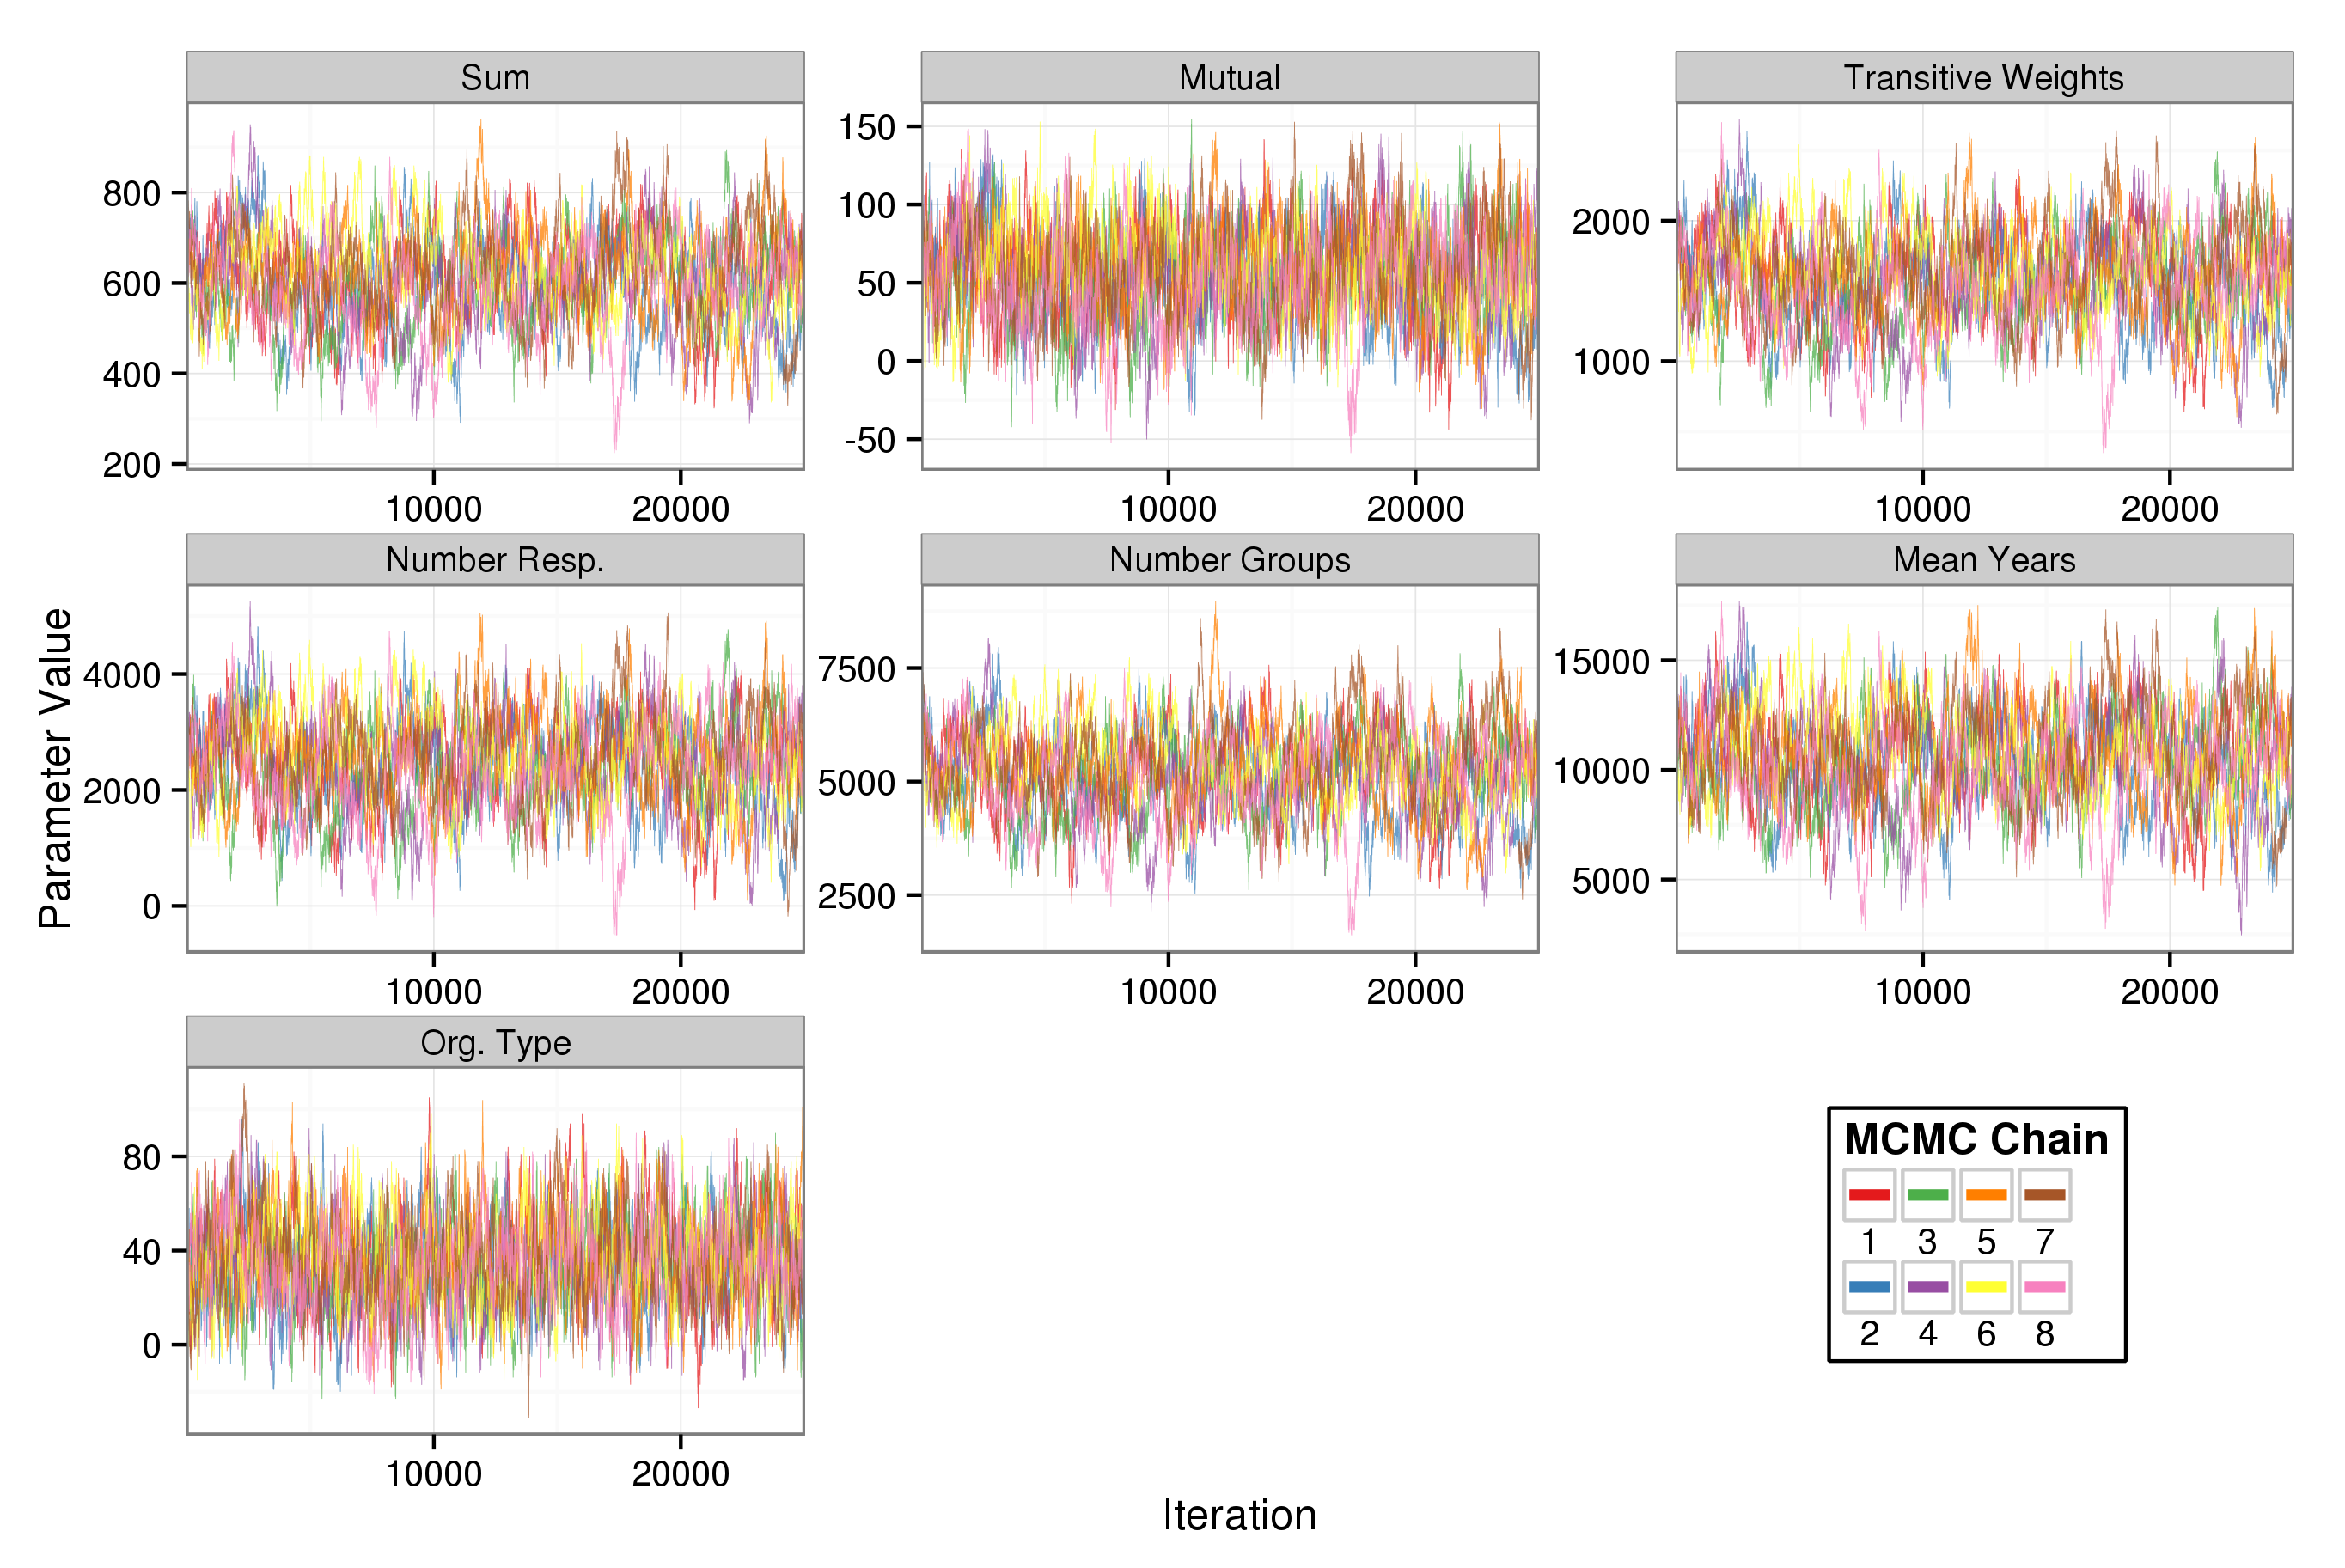
\includegraphics[width=6.5in]
{traceplotdu}
\label{figure:traceplots}
\end{figure}

Further, Figure \ref{figure:densityplots} shows smoothed parameter density plots from each MCMC run. As shown, each chain produces a unimodal distribution and generally speaking, the 8 chains produce similar distributions for each parameter. One can verify model convergence by seeing that the density plots for each parameter are normally distributed and that the respective chains for each parameter largely overlap. Ideally, the distributions for each of the 8 chains would be completely congruent; in practice, however, this is difficult to achieve for a large, non-trivial network. It is expected that were each chain run for a sufficient amount of samples, the distributions would converge. This assumption was tested by comparing the model fitting results presented in this paper to those of models with a smaller MCMC sample size; as the length of each chain increases from 1250 to 25000 (i.e., from 10,000 total samples to 200,000 total samples), the parameter distributions for each chain become more congruent. Further, it is important to note that many published ERGMs do not fit MCMC chains in parallel, and instead simply examine whether the single distribution for each parameter is normally distributed. Even though the distributions in Figure \ref{figure:densityplots} do not completely overlap, the fact that they show relatively consistent shapes and centerings across all 8 chains still serves to demonstrate more consistent, robust model behavior than does a single distribution for each parameter as produced by a standard single-chain model. 

\begin{figure}[!ht]
\caption{\textit{Density Plots of MCMC Parameters}}
\graphicspath{ {`/Users/TScott/Google\space Drive/elwha/PSJ_Submission/Version3'}}
\noindent
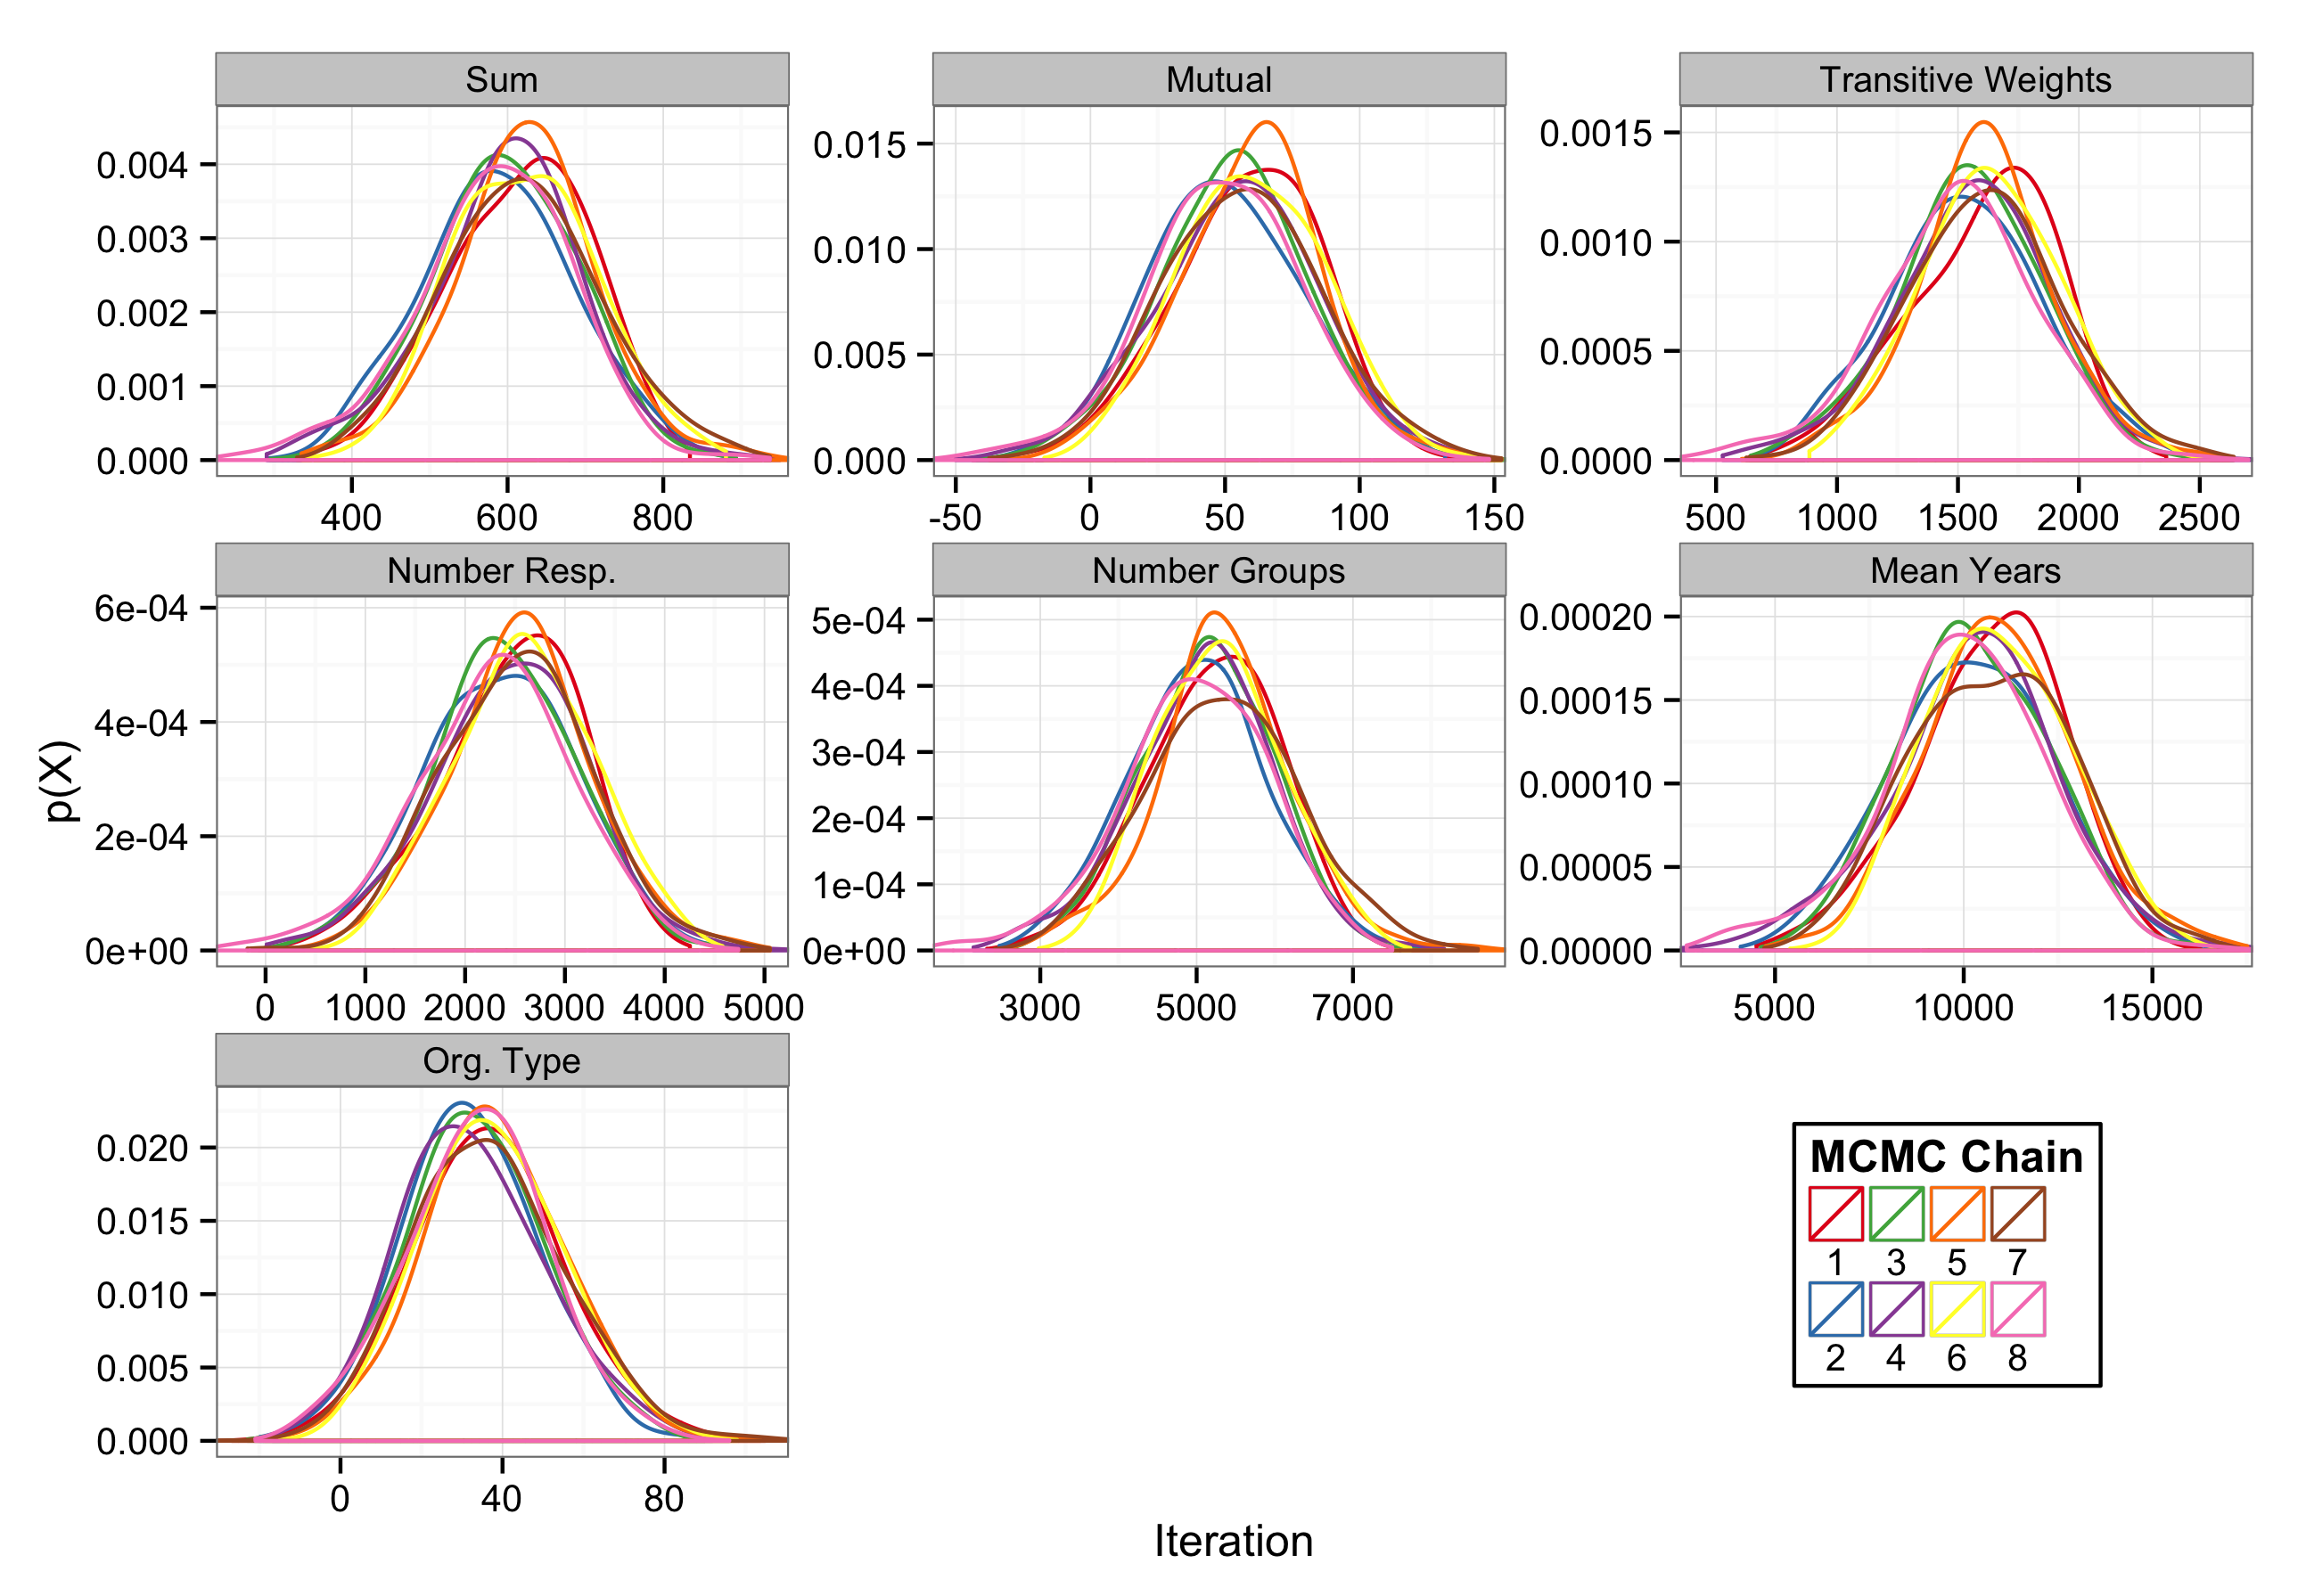
\includegraphics[width=6.5in]
{densityplotdu}
\label{figure:densityplots}
\end{figure}

One element of both Figures \ref{figure:traceplots} and \ref{figure:densityplots} the reader might notice is that the MCMC chains and parameter density plots do not necessarily center around zero. Traditionally, this has been a third aspect by which goodness-of-fit is evaluated using the \textit{statnet} package \parencite{handcock2014-a}. However, recent changes made to the \textit{ergm} package version 3.2.4 \parencite{handcock2014-a} that improve estimation and speed model fitting render zero-centering an invalid heuristic for these MCMC chain statistics. As a final test then, I also simulate a large number of networks (50,000) based upon the best-fit model and compare the distribution of statistics for these simulated network to the observed network on which the model is based. As shown in Figure \ref{figure:simplots}, the distribution of simulated statistics for each parameter is centered and neatly distributed around the observed statistic for each model parameter.

\begin{figure}[!ht]
\caption{\textit{Density of Simulated Network Statistics}}
\graphicspath{ {`/Users/TScott/Google\space Drive/elwha/PSJ_Submission/Version3'}}
\noindent
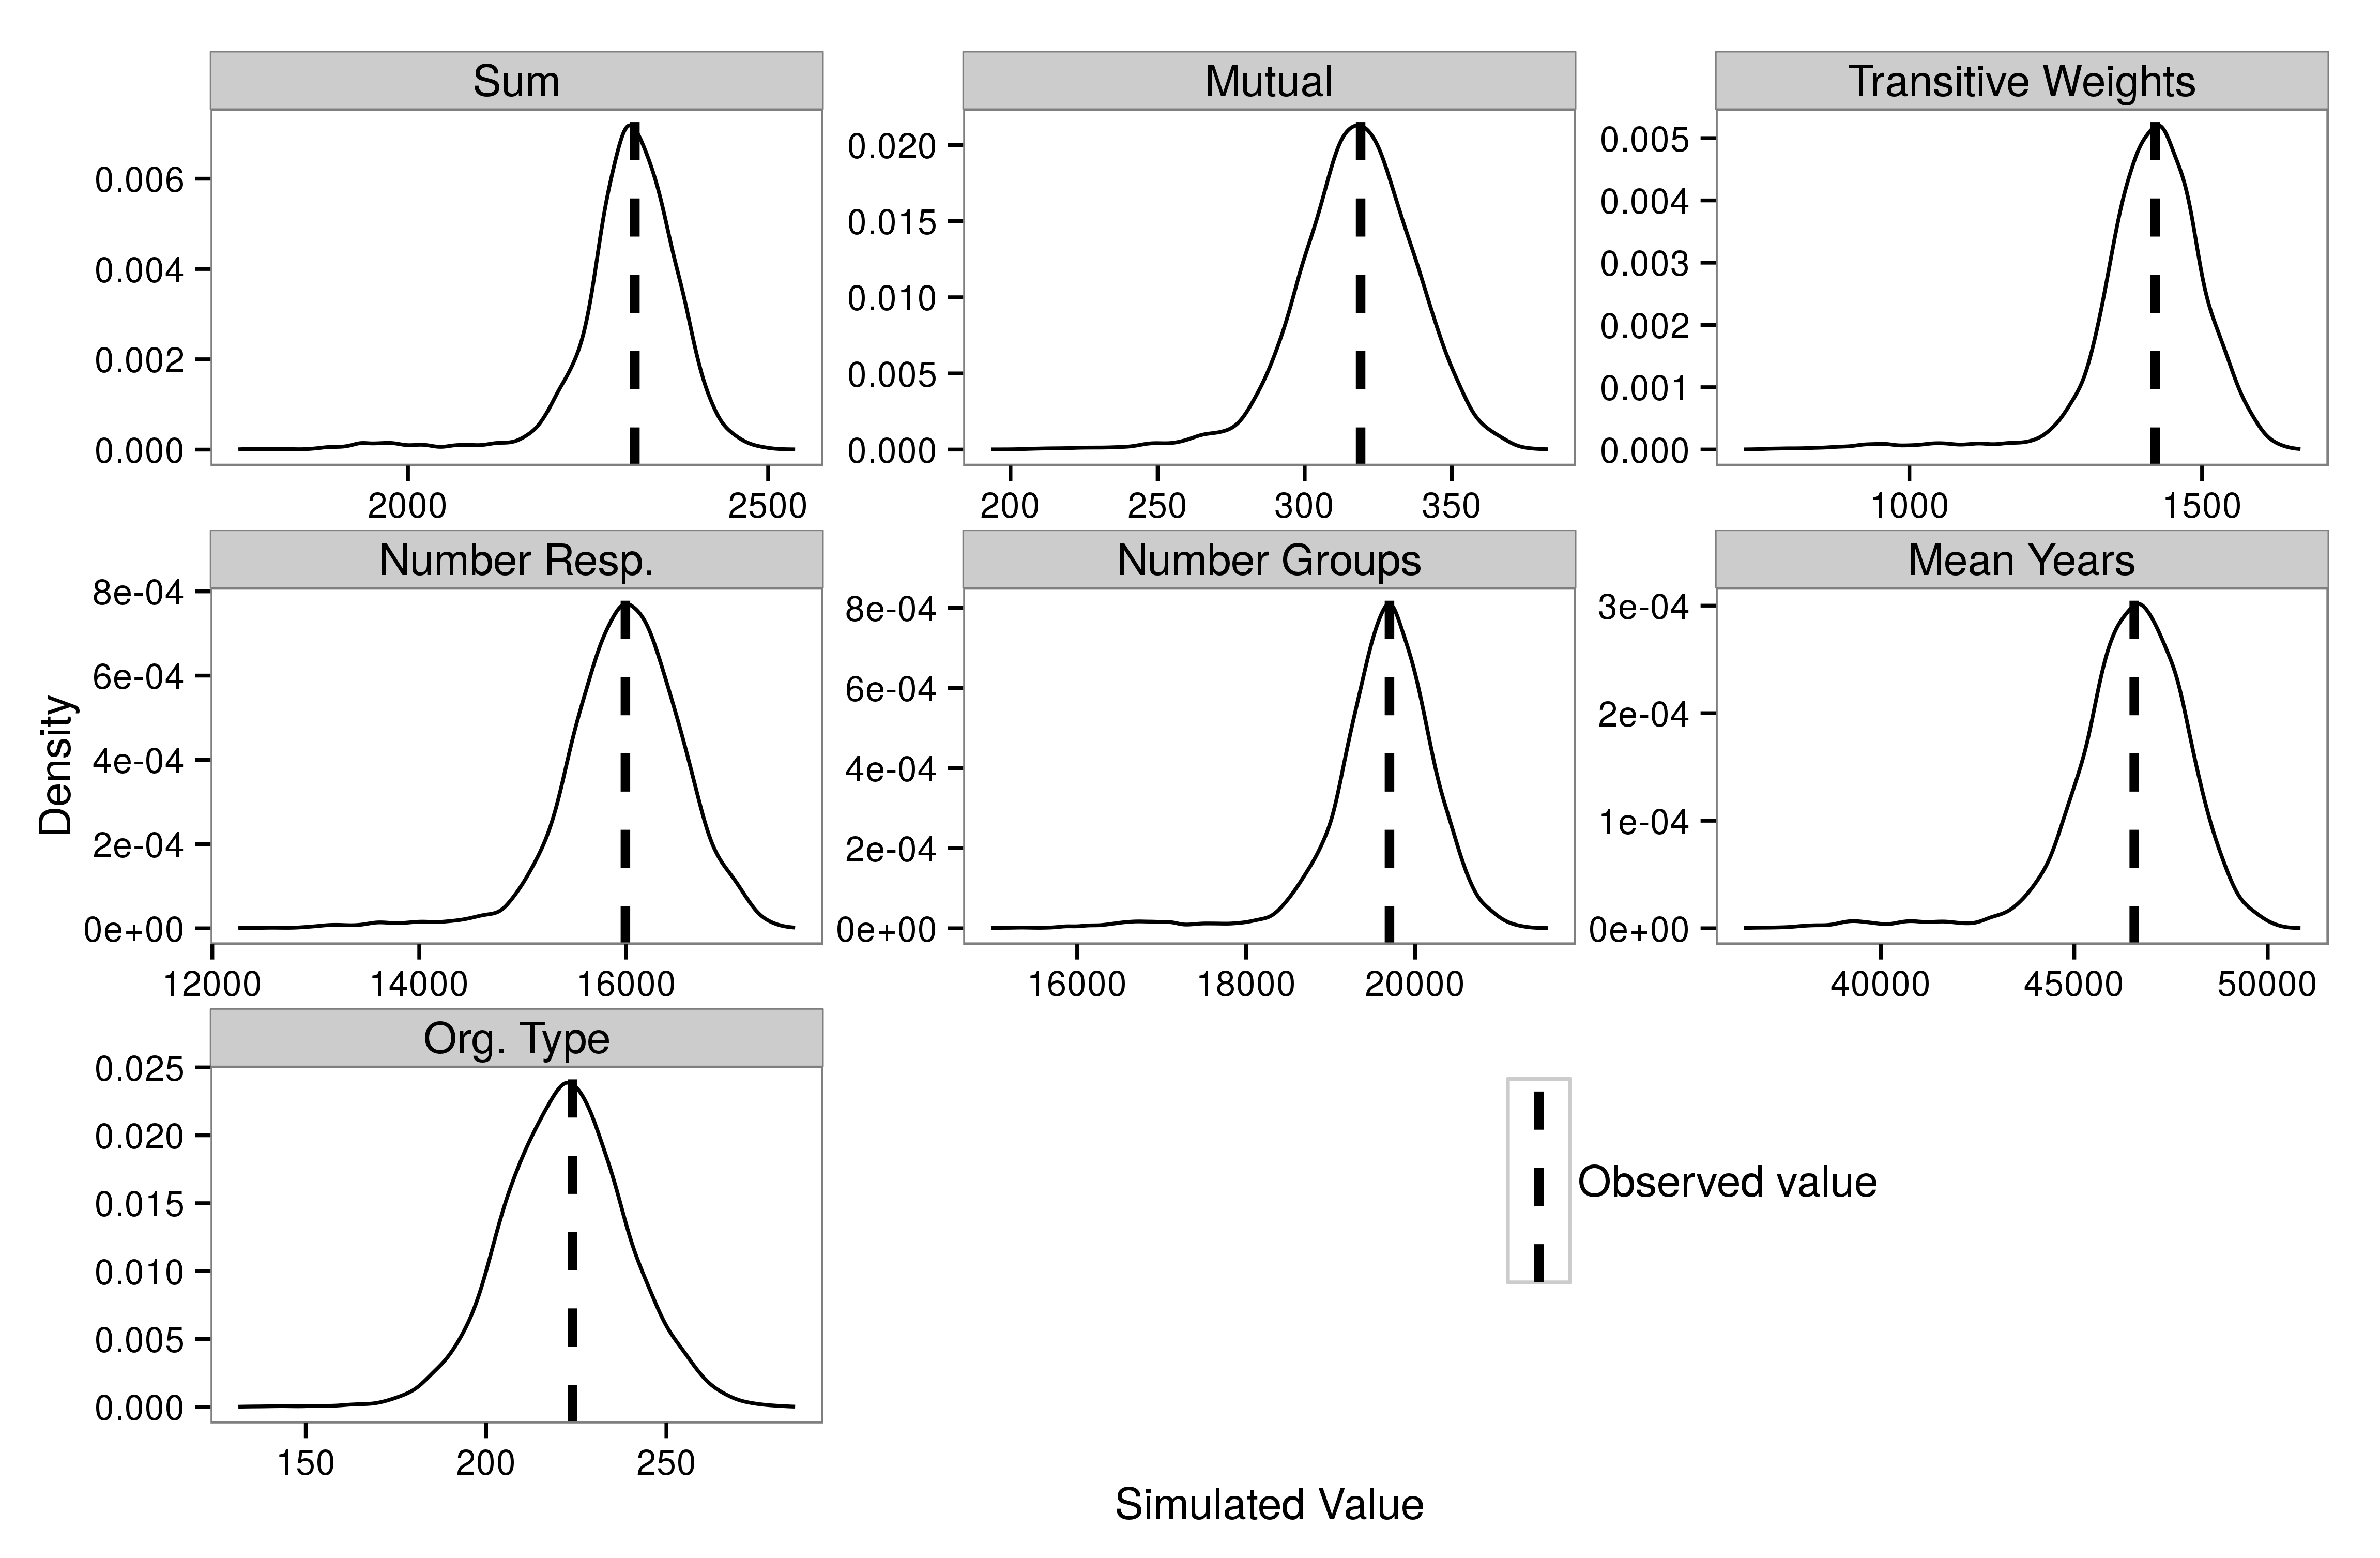
\includegraphics[width=6.5in]
{simulationplot}
\label{figure:simplots}
\end{figure}


\end{document}

































